% =============================================================================
% Lecture 05: Tree Ensembles --- Random Forests & Boosted Trees
% ECON 8310: Business Forecasting
% University of Nebraska at Omaha
% =============================================================================

\documentclass[aspectratio=169, 11pt]{beamer}

\input{header}

% ---- Lecture metadata --------------------------------------------------------
\title[Tree Ensembles]{Tree Ensembles: Random Forests \& Boosted Trees}
\subtitle{ECON 8310: Business Forecasting --- Lecture 5}
\author{Department of Economics}
\institute{University of Nebraska at Omaha}

% =============================================================================
\begin{document}
% =============================================================================

\begin{frame}
  \titlepage
\end{frame}

% ---- Outline ----------------------------------------------------------------
\begin{frame}{Lecture Outline}
  \tableofcontents
\end{frame}

% =============================================================================
\section{From Single Trees to Ensembles}
% =============================================================================

\sectionslide{From Single Trees to Ensembles}{%
  Averaging many imperfect models can outperform any single model.}

% --- Slide: Wisdom of crowds -------------------------------------------------
\begin{frame}{The Wisdom of Crowds}
  A single expert can be wrong. Average many \emph{independent} estimates and the errors tend
  to cancel.
  \begin{examplebox}{Classic Example: Guessing the Ox's Weight}
    At a 1907 county fair, 800 people guessed the weight of an ox. No individual was very
    accurate --- but the \textbf{average of all 800 guesses} came within one pound of the
    true weight.
  \end{examplebox}

  \vspace{0.15cm}
  Models work the same way. One tree is unstable, Lecture 4's closing complaint. Average many
  trees fitted to different versions of the data and the noise largely cancels while the signal
  survives.

  \vspace{0.15cm}
  \textbf{Ensembles work because independent errors cancel.} The more independent the trees, the
  more averaging removes: the difference between bagging and random forests turns on that word.
\end{frame}

% =============================================================================
\section{Bagging: Bootstrap Aggregating}
% =============================================================================

\sectionslide{Bagging: Bootstrap Aggregating}{%
  Train many trees on bootstrap samples; average their predictions.}

% --- Slide: What is bagging --------------------------------------------------
\begin{frame}{Bagging: The Big Idea}
  \textbf{Problem from Lecture 4:} one tree has high variance. \textbf{Bagging}
  \parencite{Breiman1996} averages it away:
  \begin{enumerate}\small\itemsep0pt
    \item Draw $B$ \textbf{bootstrap samples} (with replacement, the same size as the data)
    \item Fit one deep decision tree to each
    \item \textbf{Average} the $B$ predictions:
          $\hat{y}_{\text{bag}} = \tfrac{1}{B}\sum_{b=1}^{B} \hat{f}^{(b)}(\mathbf{x})$
  \end{enumerate}

  \vspace{0.1cm}
  \textbf{Why it works.} With $\rho$ the correlation between two trees' predictions,
  \[
    \Var(\bar{f}) = \rho\sigma^2 + \tfrac{1-\rho}{B}\sigma^2 .
  \]
  More trees shrink the second term; the first never moves. \textbf{That floor, $\rho\sigma^2$,
  is set by how alike the trees are}, not by how many you grow.
\end{frame}

% --- Slide: Out-of-bag error --------------------------------------------------
\begin{frame}{Out-of-Bag (OOB) Error: Free Cross-Validation}
  A bootstrap sample holds about \textbf{63\%} of the distinct rows; the rest are
  \textbf{out-of-bag} for that tree. Score each row with only the trees that never saw it: an
  out-of-sample RMSE, no refitting (\texttt{oob\_score=True}).
  \begin{warningbox}
    \textbf{On a time series it is not a forecast test.} Each row is out-of-bag for about $0.37B$
    trees whatever $n$ is; small $n$ is noisy only because there are few rows to average. Worse,
    those trees trained on the weeks \emph{after} the row: OOB scores filling a gap, not
    forecasting. Use walk-forward CV.
  \end{warningbox}
\end{frame}

% =============================================================================
\section{Random Forests: Decorrelating the Trees}
% =============================================================================

\sectionslide{Random Forests: Decorrelating the Trees}{%
  Restrict each split to a random subset of features so trees are less alike.}

% --- Slide: The correlation problem ------------------------------------------
% Figure: scripts/figures/lecture05_figures.py root_splits (Lab 5's data; numbers in measured.json).
\begin{frame}{The Problem Bagging Does Not Fully Solve}
  If one feature dominates (\texttt{dow} daily, the four-week lag weekly), nearly every bagged
  tree splits on it first and $\rho$ stays high. \textbf{The random forest fix}
  \parencite{Breiman2001}: at each split, consider only a random $m < p$ of the features.
  \begin{center}
    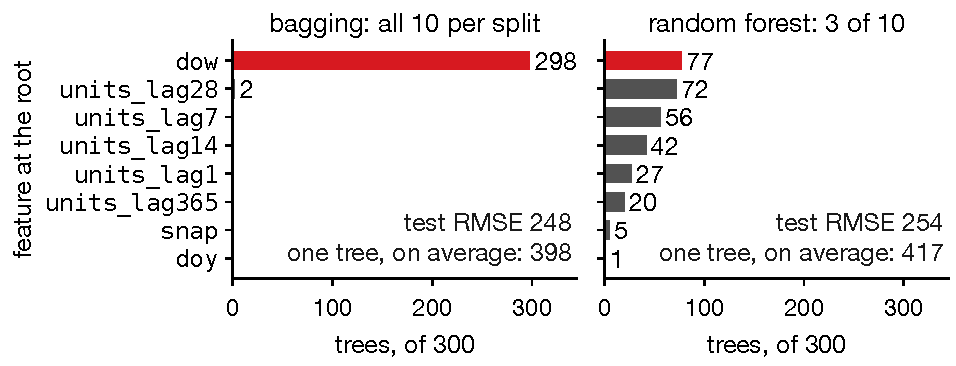
\includegraphics[height=4.0cm]{../Figures/Lecture05_TreeEnsembles/root_splits.pdf}
  \end{center}
  \vspace{-0.3cm}
  {\small Lab 5, 300 trees each. The fix spreads the roots, and its trees average better (417 to
  254, against 398 to 248), but they start worse: with one dominant feature among ten,
  \texttt{sqrt} loses.}
\end{frame}

% --- Slide: RF hyperparameters -----------------------------------------------
\begin{frame}{Random Forest Hyperparameters}
  \begin{center}
    {\footnotesize
    \begin{tabular}{p{3.0cm}p{2.8cm}p{1.8cm}p{4.0cm}}
      \toprule
      \textbf{Parameter} & \textbf{sklearn name} & \textbf{Default} & \textbf{Effect} \\
      \midrule
      Number of trees & \texttt{n\_estimators} & 100 & More = lower variance; plateaus $\sim$500 \\
      Max features/split & \texttt{max\_features} & \texttt{1.0} (all) & Lower = more decorrelated \\
      Max depth & \texttt{max\_depth} & None & Limit only to reduce memory \\
      Min samples/leaf & \texttt{min\_samples\_leaf} & 1 & Higher = smoother predictions \\
      OOB score & \texttt{oob\_score} & False & \texttt{True} gives a free CV estimate \\
      \bottomrule
    \end{tabular}
    }
  \end{center}

  \textbf{The default is plain bagging.} scikit-learn's regressor considers every feature at
  every split; \texttt{'sqrt'} is the classifier's default. So set \texttt{max\_features}
  yourself: it is the dial for $\rho$, and the only one that really needs tuning. Start with
  \texttt{n\_estimators=500}, \texttt{min\_samples\_leaf=5}.

  \muted{\footnotesize Set \texttt{random\_state=42}: a forest is random twice over, in the
  bootstrap samples and in the feature subsets.}
\end{frame}

% =============================================================================
\section{Feature Importance and Interpretation}
% =============================================================================

\sectionslide{Feature Importance and Interpretation}{%
  Which predictors matter most? RF gives a data-driven answer.}

% --- Slide: Feature importance -----------------------------------------------
\begin{frame}{Random Forest Feature Importance \parencite{Molnar2022}}
  \begin{definitionbox}{Mean Decrease in Impurity (MDI)}
    \small For each feature $j$, average the total reduction in node impurity across every
    split on $j$, weighted by the fraction of observations reaching that node. Normalize to
    sum to 1.
  \end{definitionbox}
  \begin{center}
    {\small
    \begin{tabular}{lc}
      \toprule
      \textbf{Feature (CA\_1 FOODS, weekly)} & \textbf{Importance} \\
      \midrule
      \texttt{units\_lag4}  & 0.28 \\
      \texttt{units\_lag1}  & 0.21 \\
      \texttt{snap\_days}   & 0.17 \\
      \texttt{units\_lag52} & 0.15 \\
      \texttt{units\_lag2}  & 0.09 \\
      \texttt{units\_lag3}  & 0.06 \\
      \bottomrule
    \end{tabular}
    }
  \end{center}

  From the next slide's forest; Lecture 4's single tree gave the four-week lag 0.62. A screening
  device only: \textbf{MDI is biased} toward features with many split points.
  \texttt{permutation\_importance} (shuffle a column, measure the damage) is the honest
  alternative.
\end{frame}

% --- Slide: Python implementation -----------------------------------------
\begin{frame}{Random Forest in Python}
  \begin{examplebox}{sklearn Code Template}
    {\scriptsize
    \texttt{from sklearn.ensemble import RandomForestRegressor}\\
    \texttt{rf = RandomForestRegressor(n\_estimators=500, max\_features='sqrt',}\\
    \texttt{\ \ \ min\_samples\_leaf=5, oob\_score=True, random\_state=42).fit(X\_tr, y\_tr)}\\
    \texttt{print(rf.oob\_score\_);\ \ importances = rf.feature\_importances\_}
    }
  \end{examplebox}
  \begin{center}
    {\footnotesize
    \begin{tabular}{lc}
      \toprule
      \textbf{Model (CA\_1 FOODS, 52-week test)} & \textbf{Test RMSE} \\
      \midrule
      Seasonal na\"{i}ve   & 1,660 \\
      Single deep tree     & 1,456 \\
      \textbf{Random Forest} & \textbf{1,115} \\
      \bottomrule
    \end{tabular}
    }
  \end{center}

  The forest cuts RMSE by \textbf{23\%} against a single deep tree. Both tree models beat the
  seasonal naive benchmark, the first in this course to do so on this series.

  \muted{\footnotesize What changed is not a better model of the series but a richer feature
  set --- lags, price, and SNAP days are information ETS and ARIMA never had.}
\end{frame}

% =============================================================================
\section{Gradient Boosting}
% =============================================================================

\sectionslide{Gradient Boosting}{%
  Instead of averaging independent trees, fit each new tree to the errors
  of all previous trees.}

% --- Slide: Boosting vs. bagging ---------------------------------------------
\begin{frame}{Boosting vs.\ Bagging: The Core Difference}
  \begin{columns}[T]
    \begin{column}{0.48\textwidth}
      \textbf{Bagging (Random Forest):}
      \begin{itemize}\small\itemsep0pt
        \item Trees built \textbf{in parallel}
        \item Each tree predicts $y$
        \item Averaging cuts \emph{variance}
        \item More trees never cut bias
      \end{itemize}
    \end{column}
    \begin{column}{0.48\textwidth}
      \textbf{Boosting:}
      \begin{itemize}\small\itemsep0pt
        \item Trees built \textbf{in sequence}
        \item Each fits the \emph{errors} so far
        \item Cuts \emph{bias} as well
        \item Overfits if trees are too deep or too many
      \end{itemize}
    \end{column}
  \end{columns}

  \vspace{0.2cm}
  \textbf{The intuition.} Forecast 1 says \$50,000 against an actual \$60,000; forecast 2
  predicts the \emph{error}, $+$\$10,000, and the sum is right. Each stage corrects what
  remains, fixing a bias that averaging never touches.
\end{frame}

% --- Slide: Boosting algorithm -----------------------------------------------
\begin{frame}{The Gradient Boosting Algorithm}
  \begin{definitionbox}{Gradient Boosting (squared-error loss)}
    {\footnotesize
    Initialize $F_0(\mathbf{x}) = \bar{y}$. For $b = 1, \ldots, B$:
    \begin{enumerate}\itemsep0pt\topsep0pt
      \item Compute residuals: $r_i^{(b)} = y_i - F_{b-1}(\mathbf{x}_i)$
      \item Fit a shallow tree $T_b$ to $\{(\mathbf{x}_i, r_i^{(b)})\}$
      \item Update: $F_b = F_{b-1} + \eta\, T_b$
    \end{enumerate}
    Final prediction: $\hat{y} = F_B(\mathbf{x})$
    }
  \end{definitionbox}
  Trees are \textbf{shallow} (depth 3 to 6): each captures a little of what remains.

  \vspace{0.15cm}
  \textbf{The learning rate $\eta$ is the main dial:} 0.01--0.1 is slow and robust, above 0.3
  risks overshooting. Use a small $\eta$, many trees and \textbf{early stopping}, or boosting
  fits your noise.
\end{frame}

% =============================================================================
\section{XGBoost}
% =============================================================================

\sectionslide{XGBoost}{%
  Three improvements over vanilla boosting: second-order optimization,
  explicit regularization, and column subsampling.}

% --- Slide: XGBoost innovations -----------------------------------------------
\begin{frame}{XGBoost: Three Advances \parencite{Chen2016}}
  \begin{enumerate}\itemsep3pt
    \item \textbf{Newton step.} Uses the loss's curvature as well as its slope. For squared
          error the curvature is constant, so this is the ordinary residual fit; it matters for
          log-loss or Poisson.
    \item \textbf{Explicit regularization.} Penalties on leaf count and leaf size, inside the
          objective.
    \item \textbf{Column subsampling}, borrowed from random forests.
  \end{enumerate}

  \vspace{0.15cm}
  \texttt{reg\_lambda} is Ridge and \texttt{reg\_alpha} is LASSO, on leaf weights (next week).
  \texttt{gamma} is a price per leaf, like Lecture 4's \texttt{ccp\_alpha}.

  \vspace{0.15cm}
  \muted{\small XGBoost dominated Kaggle tabular competitions in 2014--2018.}
\end{frame}

% --- Slide: XGBoost key hyperparameters --------------------------------------
\begin{frame}{XGBoost: Key Hyperparameters}
  \begin{center}
    {\footnotesize
    \begin{tabular}{p{2.6cm}p{2.8cm}p{1.8cm}p{4.0cm}}
      \toprule
      \textbf{Parameter} & \textbf{XGB name} & \textbf{Typical} & \textbf{Effect} \\
      \midrule
      Number of trees & \texttt{n\_estimators} & 500--2000 & More + small $\eta$ = better (use early stopping) \\
      Learning rate & \texttt{learning\_rate} & 0.01--0.1 & Smaller = more robust; needs more trees \\
      Tree depth & \texttt{max\_depth} & 3--6 & Shallow preferred; depth $>$6 risks overfit \\
      Row subsample & \texttt{subsample} & 0.7--0.9 & Fraction of training rows per tree \\
      Col.\ subsample & \texttt{colsample\_bytree} & 0.7--0.9 & Feature fraction per tree (like RF) \\
      L2 leaf penalty & \texttt{reg\_lambda} & 1 & Ridge on leaf weights; stabilizes \\
      \bottomrule
    \end{tabular}
    }
  \end{center}
  \begin{keybox}
    \small \textbf{Practical starting point:}
    \texttt{learning\_rate=0.05}, \texttt{max\_depth=4},
    \texttt{n\_estimators=1000} with early stopping on validation RMSE.
    Tune \texttt{max\_depth} and \texttt{subsample} via \texttt{TimeSeriesSplit}.
  \end{keybox}
\end{frame}

% --- Slide: XGBoost Python ---------------------------------------------------
\begin{frame}{XGBoost in Python}
  \begin{examplebox}{Code Template}
    {\scriptsize
    \texttt{model = xgb.XGBRegressor(n\_estimators=1000, learning\_rate=0.05,}\\
    \texttt{\ \ max\_depth=4, subsample=0.8, colsample\_bytree=0.8,}\\
    \texttt{\ \ early\_stopping\_rounds=50, random\_state=42)}\\
    \texttt{model.fit(X\_train, y\_train, eval\_set=[(X\_val, y\_val)], verbose=False)}
    }
  \end{examplebox}
  \texttt{eval\_set} is what makes \texttt{early\_stopping\_rounds} work: XGBoost watches
  validation RMSE and halts when it stops improving, which is how you get away with setting
  \texttt{n\_estimators} far higher than you need.

  \textbf{The validation set must respect time.} Build it with \texttt{TimeSeriesSplit} and
  hold out the final stretch as a true test set.

  \muted{\footnotesize On macOS \texttt{xgboost} also needs OpenMP:
  \texttt{brew install libomp}, or the import fails.}
\end{frame}

% =============================================================================
\section{Key Takeaways and Roadmap}
% =============================================================================

\sectionslide{Key Takeaways and Roadmap}{%
  Bagging reduces variance; boosting reduces bias. Together they cover
  most of what tabular forecasting needs.}

% --- Slide: Which method when -------------------------------------------------
\begin{frame}{Tree Methods: Which One When}
  \begin{center}
    {\small
    \begin{tabular}{lllll}
      \toprule
      \textbf{Method} & \textbf{Training} & \textbf{Interpretable} & \textbf{Tuning} & \textbf{Accuracy} \\
      \midrule
      Decision Tree & Single tree & High & Low & Baseline \\
      Random Forest & Parallel ($B$ trees) & Medium & Low & Good \\
      XGBoost & Sequential ($B$ trees) & Low & Higher & Best \\
      \bottomrule
    \end{tabular}
    }
  \end{center}

  \textbf{Random Forest is the better default}: robust, almost no tuning, OOB error for free.
  \textbf{Move to XGBoost} when you can afford to tune and need the last few points --- and
  budget for that tuning, because an untuned XGBoost often loses to a default forest.
\end{frame}

% --- Slide: no tree can extrapolate ------------------------------------------
% Figure: scripts/figures/lecture05_figures.py extrapolation (numbers in measured.json, "rsxfs").
\begin{frame}{Why No Tree Can Extrapolate}
  A forest's prediction is a weighted average of training targets, so it can never leave
  [training min, training max]. A forest trained on US retail sales through 2019, then given each
  later month's true lags:
  \begin{center}
    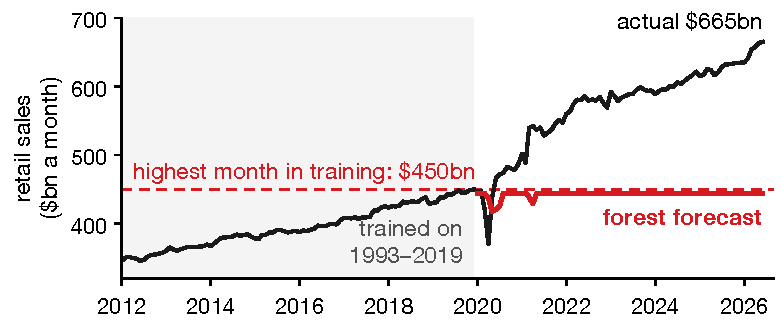
\includegraphics[height=4.0cm]{../Figures/Lecture05_TreeEnsembles/extrapolation.pdf}
  \end{center}
  \vspace{-0.3cm}
  {\small It never forecasts above \$450bn; by mid-2026 sales are \$665bn. Boosted trees go flat
  beyond their last split too. On a trending series, keep a model that can extrapolate.}
\end{frame}

% --- Slide: Key takeaways ---------------------------------------------------
\begin{frame}{Lecture 5: Key Takeaways}
  \begin{keybox}
    {\small
    \begin{enumerate}\itemsep2pt
      \item \textbf{Ensembles} work because independent errors cancel.
      \item \textbf{Bagging} averages bootstrap trees; variance floors at $\rho\sigma^2$.
      \item \textbf{Random forests} cut $\rho$ by sampling features at each split --- when no
            single feature dominates.
      \item \textbf{OOB error} is free, but on a time series it scores gaps, not forecasts.
      \item \textbf{Boosting} fits each tree to the errors so far: it attacks bias.
      \item No tree can \textbf{extrapolate} beyond the training range.
      \item Tune with \texttt{TimeSeriesSplit}; pair boosting with \textbf{early stopping}.
    \end{enumerate}
    }
  \end{keybox}
  \muted{\itshape Next: Regularization \& Model Selection ---
  choosing among many predictors by shrinking coefficients rather than counting them.}
\end{frame}

% --- References ---------------------------------------------------------------
\begin{frame}[allowframebreaks]{References}
  \printbibliography[heading=none]
\end{frame}

% =============================================================================
\end{document}
% =============================================================================
